\let\negmedspace\undefined
\let\negthickspace\undefined
\documentclass[journal,12pt,twocolumn]{IEEEtran}
\usepackage{gensymb}
\usepackage{amssymb}
\usepackage{enumitem}
\usepackage{graphicx}
\usepackage{amsmath}
\begin{document}
\graphicspath{{figures/}}

\title{Assignment 2 \\ \Large AI1110: Probability and Random Variables \\ \large Indian Institute of Technology Hyderabad}
\author{Kushagra Gupta \\ \normalsize CS21BTECH11033  \\ \Large ICSE 2018 Grade 12}
\date{}
\maketitle
\begin{flushleft}
\textbf{Q8-a:}
Find the points on the curve $y = 4x^3 - 3x + 5$ at which the equation of the tangent is parallel to $x-axis$

%\textbf{Solution:} We know that the slope of x-axis $= 0$ so any tangent line parallel to it must have %slope $=0$.\\ We also know that the first derivative of a function gives us a function for slope of %tangent at all points in domain. As $y = f(x)$  is a polynomial function, $f(x)$ is differentiable at %all points in domain and hence first derivative exists.
\textbf{Solution: }$y = f(x)$ is differentiable, and the derivative represents the tangent at a point in $f$. Since any tangent parallel to the $x-axis$ has slope $0$, we equate $f'(x)$ to $0$

\begin{align}
    &y = f(x) = 4x^3 - 3x + 5\\
    &\Rightarrow \frac{dy}{dx} = f'(x) = \frac{d}{dx}(4x^3 - 3x + 5) \\
    &\Rightarrow f'(x) = 12x^2 - 3 
\end{align} 

We want roots for $f'(x) = 0$.

\begin{align}
    &\therefore f'(x) = 12x^2 - 3 = 0 \\
    &\Rightarrow x^2 = \frac{1}{4}\\
    &\Rightarrow x = \pm \sqrt{\frac{1}{4}}\\
    &\Rightarrow x = \pm \frac{1}{2} 
\end{align}

Now at $ x = \pm \frac{1}{2}$ we get from equation $(1)$,
\begin{align}
    &y =  4 \times\left(\pm\frac{1}{2}\right)^3 - 3\times\left(\pm\frac{1}{2}\right) + 5\\
    &\Rightarrow y = \pm\frac{1}{2} \mp\frac{3}{2} + 5\\
    &\Rightarrow y = 4 , 6
\end{align}
$\therefore$ At  $(x,y) = \left(\frac{1}{2},4\right) , \left(\frac{-1}{2},6\right)$ the tangents are parallel to x axis.\\

\begin{figure}[!ht]
		\centering
		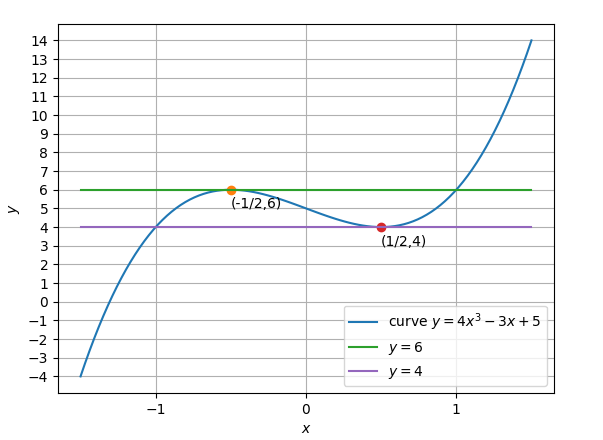
\includegraphics[width=\columnwidth]{figures/plot.png}
		\caption{Plot showing curve and appropriate tangents}
		\label{plot}
\end{figure}

\end{flushleft}
\end{document}
